\section{Applications Of Fractional Calculus}
Fractional differential equations and integral equations appear in several physical systems
In this section we will review some of their applications.


\subsection{Abel's Fractional Integral Equation Of Tautochrone}
The Abel's problem is to find a curve where the time that takes a ball to reach the bottom of the curve is same irrespective 
of the position of release of ball in friction less system. 

\begin{figure*}[h]
    \hspace*{1cm}
    \begin{minipage}[l]{.5\textwidth}
        \begin{tikzpicture}
            \draw[->] (0,0) -- (0,3);
            \draw[->] (0,0) -- (pi+1,0);
            \draw[red,domain=pi:2*pi,samples=50] plot ({-(\x - sin(\x r))+2*pi},{-(1 - cos(\x r))+2});
            
            \filldraw [blue] (0,2) circle (2pt);
            \filldraw [green] (.5,1.07) circle (2pt);
            \filldraw [yellow] (1.3,.47) circle (2pt);
            \filldraw [red!50!blue] (2,.17) circle (2pt);
            \node at (2, 2) {$t = t_i$};
        \end{tikzpicture}
    \end{minipage}  
    \begin{minipage}[r]{.5\textwidth}
        \begin{tikzpicture}
            \draw[->] (0,0) -- (0,3);
            \draw[->] (0,0) -- (pi+1,0);
            \draw[red,domain=pi:2*pi,samples=50] plot ({-(\x - sin(\x r))+2*pi},{-(1 - cos(\x r))+2});
            
            \filldraw [blue] (pi,0) circle (2pt);
            \filldraw [green] (pi,0) circle (2pt);
            \filldraw [yellow] (pi,0) circle (2pt);
            \filldraw [red!50!blue] (pi,0) circle (2pt);
            \node at (2, 2) {$t = t_f$};
        \end{tikzpicture}
    \end{minipage} 
\end{figure*}

Let $S$ be the arc length measured along curve $C$ from point $O$ to an arbitrary point $Q$ on $C$
\begin{center}
    \begin{tikzpicture}
        \draw[->] (0,0) -- (0,3);
        \draw[->] (0,0) -- (pi+1,0);
        \draw[red,domain=pi:2*pi,samples=50] plot ({-(\x - sin(\x r))+2*pi},{-(1 - cos(\x r))+2});
        
        \draw[green,domain=pi:1.52*pi,samples=50] plot ({-(\x - sin(\x r))+2*pi},{-(1 - cos(\x r))+2});
        \filldraw [blue] (.5,1.07) circle (2pt);
        \node at (1.5, .8) {$S$};
        \node at (pi, -.2) {$O$};
        \node at (-.2, 2) {$P$};
        \node at (.5, .5) {$C$};
        \node at (.8,1.2) {$Q$};
    \end{tikzpicture}
\end{center}
The gain in Kinetic Energy while the ball descends is loss in the
potential energy and is given by
\begin{align*}
    \frac{1}{2}m \left(\dv{s}{t}\right)^2 &= mg(y-\eta)
    \\
    ds &= - \sqrt{2g (y-\eta)} \hquad dt
\end{align*}
The negative square root indicates that the distance (arc-length) decreases as the
time increases.
The equation thus to be solved is
\[
    dt = -\frac{1}{\sqrt{2g (y-\eta)}} \hquad ds
\]
The time of decent from $P$ to $O$ is $T$ , which is constant thus
\[
    T = -\frac{1}{\sqrt{2g}} \int_{P}^{O}\frac{1}{\sqrt{(y-\eta)}} \hquad ds
\]
Now taking, the arc length as a function $s = h(\eta)$ , where $h$ depends on the shape
of $C$. \\
We can write in differential form the curve as $\displaystyle ds = \dv{}{\eta}h(\eta) \hquad d\eta $ , so this substitution gives
\begin{align*}
    T &= -\frac{1}{\sqrt{2g}} \int_{y}^{0}\frac{1}{\sqrt{(y-\eta)}} \dv{}{\eta}h(\eta) \hquad d\eta
    \\
    \sqrt{2g} T &= \int_{0}^{y}(y-\eta)^{-\frac{1}{2}} \dv{}{\eta}h(\eta) \hquad d\eta
\end{align*}
Meaning that the integral of right hand side of above, when a constant will be solution to get
constant time of decent $(T)$. In the above expression rewriting the integral of right hand side as
\[
    \sqrt{2g} T = \int_{0}^{y}(y-t)^{-\frac{1}{2}} f(t) \hquad dt
\]
This is Abel's integral equation where $\displaystyle f(t) = \dv{}{t}h(t)$.
\\
Abel solved this problem using convolutions and Laplace transforms but using fractional calculus 
we can see a much quicker solution if we divide both sides by $\Gamma(\frac{1}{2})$ which is equal to $\sqrt{\pi}$
we get this 
\[
    \frac{\sqrt{2g}}{\sqrt{\pi}} T = \frac{1}{\Gamma(\frac{1}{2})} \int_{0}^{y}(y-t)^{-\frac{1}{2}} f(t) \hquad dt
\]
We notice that the integral in the right hand side is the semi integral of $f(t)$
\\
In terms of fractional order Integral, this equation can be written as
\[
    \sqrt{\frac{2g}{\pi}} T = I^{\frac{1}{2}}f(t)
\]
Now by taking half derivative of RL type for both sides we get 
\[
    D^{\frac{1}{2}} \sqrt{\frac{2g}{\pi}} T = f(t)
\]
Thus 
\[
    f(t) = \sqrt{\frac{2g}{\pi}} \frac{T}{\sqrt{t}}
\]
Doing algebraic manipulation the following is obtained.
\[
    f(y) = \dv{}{y} h(y) = \dv{s}{y} = \frac{\sqrt{dx^2 + dy^2}}{dy} = \sqrt{1+ \left(\dv{x}{y}\right)^2}
\]
Thus
\begin{align*}
    \dv{x}{y} &= \sqrt{f(y)^2-1}
    \\
    x &= \int_{0}^{y} \sqrt{\frac{2g T^2}{\pi^2 \eta} - 1} \hquad d\eta + C
\end{align*}
If we make the curve start from (0,0)

\begin{center}
    \begin{tikzpicture}
        \draw[->] (0,0) -- (0,3);
        \draw[->] (0,0) -- (3,0);
        \draw[red,domain=0:pi,samples=50] plot ({\x - sin(\x r)},{1 - cos(\x r)});
    \end{tikzpicture}
\end{center}

We can get that $C = 0$

Now Substitute \(
    \begin{cases}
        \displaystyle a = \frac{2g T^2}{\pi^2}
        \\
        \displaystyle \eta = 2a \hquad sin^2(\xi)
        \\
        \displaystyle d\eta = 4a \hquad sin(\xi) \hquad cos(\xi) \hquad d\xi
        \\
        \displaystyle 0 \to \beta
        \\
        \displaystyle \beta = sin^{-1}\left(\sqrt{\frac{y}{2a}}\right)
    \end{cases}
    \)
\\
We get 
\begin{align*}
    x &= 4a \int_{0}^{\beta} \sqrt{\csc^2(\xi) - 1} \hquad sin(\xi) \hquad cos(\xi) \hquad d\xi
    \\
    x &= 4a \int_{0}^{\beta} \cot(\xi) \hquad sin(\xi) \hquad cos(\xi) \hquad d\xi
    \\
    x &= 4a \int_{0}^{\beta} cos^2(\xi) \hquad d\xi
\end{align*}
Thus we obtain
\begin{align*}
    x &= 2a\left(\beta - \frac{1}{2}\sin(2\beta)\right)
    \\
    y &= 2a\sin^2(\beta)
\end{align*}
Put $\theta = 2\beta$ and we know that $\displaystyle a=\frac{gT^2}{\pi^2}$ we obtain
\begin{align*}
    x &= a\left(\theta - \sin(\theta)\right)
    \\
    y &= a(1-\cos(\theta))
\end{align*}
The parametric equation of the cycloid
\\
The cycloid is a curve you get when you roll a circle and focus on a point 
\begin{center}
    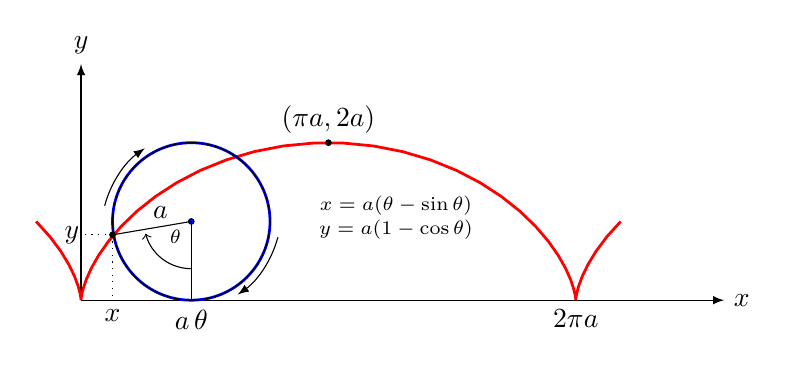
\begin{tikzpicture}
    \coordinate (O) at (0,0);
    \coordinate (A) at (0,3);
    \def\r{1} % radius
    \def\c{1.4} % center
    \coordinate (C) at (\c, \r);
  
  
    \draw[-latex] (O) -- (A) node[anchor=south] {$y$};
    \draw[-latex] (O) -- (2.6*pi,0) node[anchor=west] {$x$};
    \draw[red,domain=-0.5*pi:2.5*pi,samples=50, line width=1] 
         plot ({\x - sin(\x r)},{1 - cos(\x r)});
    \draw[blue, line width=1] (C) circle (\r);
    \draw[] (C) circle (\r);
  
    % coordinate x 
    \def\x{0.4} % coordinate x
    \def\y{0.83} % coordinate y
    \def\xa{0.3} % coordinate x for arc left
    \def\ya{1.2} % coordinate y for arc left
    \coordinate (X) at (\x, 0 );
    \coordinate (Y) at (0, \y );
    \coordinate (XY) at (\x, \y );
  
    \node[anchor=north] at (X) {$x$} ;
  
    % draw center of circle
    \draw[fill=blue] (C) circle (1pt);
  
    % draw radius of the circle
    \draw[] (C) -- node[anchor=south] {\; $a$} (XY);
  
    % bottom of circle, radius to the bottom
    \coordinate (B) at (\c, 0);
    \draw[] (C) -- (B) node[anchor=north] {$a \, \theta$};
  
    % projections of point XY
    \draw[dotted] (XY) -- (X);
    \draw[dotted] (XY) -- (Y) node[anchor=east, xshift=1mm] {$\quad y$};
  
    % arc theta
    % start arc
    \coordinate (S) at (\c, 0.4);
    \draw[->] (S) arc (-90:-165:0.6);
    \node[xshift=-2mm, yshift=-2mm] at (C) {\scriptsize $\theta$};
  
    % arc above
    \coordinate (AA) at (\xa, \ya);
    \draw[-latex, rotate=25] (AA) arc (-220:-260:1.3);
  
    % arc below
    \def\xb{2.5} % coordinate x for arc bottom
    \def\yb{0.8} % coordinate y for arc bottom
    \coordinate (AB) at (\xb, \yb);
    \draw[-latex, rotate=-10] (AB) arc (-5:-45:1.3);
  
  
  
    % XY dot
    \draw[fill=black] (XY) circle (1pt);
  
  
    % top label
    \coordinate (T) at (pi, 2);
    \node[anchor=south] at (T)  {$(\pi a, 2 a )$} ;
    \draw[fill=black] (T) circle (1pt);
  
    % equations
    \coordinate (E) at ( 4,1.2);
    \coordinate (F) at ( 4,0.9);
    \node[] at (E) {\scriptsize $x=a(\theta - \sin \theta)$};
    \node[] at (F) {\scriptsize $y=a(1 - \cos \theta)$};
  
    % label 2pi a
    \coordinate (TPA) at (2*pi, 0);
    \node[anchor=north] at (TPA) {$2 \pi a$};
  
  
    \end{tikzpicture}
  \end{center}
Cycloid is the tautochrone.
\\
A point be mentioned about the cycloid curve shape is that this is too a
curve for brachistochrone problem solved by Bernoulli. That is determination of
shape of the curve giving minimum time of descent. Therefore, the constant time
$T$ is also minimum time of descent in a cycloid.

\subsection{Viscoelasticity}
Viscoelasticity is a the field that interested in studying the property of materials that exhibit 
both viscous and elastic characteristics when undergoing deformation
and it seems to be the field of the most extensive applications
of fractional differential and integral operators.

There are two main quantities in viscoelasticity, a stress $\sigma(t)$ and a strain $\epsilon(t)$.
\\
The relationships between stress and strain for solids(Hooke’s law)
\[
\sigma(t) = E\epsilon(t)   
\]
And for Newtonian fluids
\[
\sigma(t) = \eta \dv{\epsilon(t)}{t}   
\]
Where $E$ and $\eta$ are constants. These functions satisfy the fractional
differential equations
\[
    D^\alpha \sigma(t) = \frac{\Gamma(1-\alpha) t^{-\alpha}}{\Gamma(1-2\alpha)} \sigma(t)
\]
\[
    D^\alpha \epsilon(t) = \Gamma(1+\alpha)t^{-\alpha} \epsilon(t)
\]
\newpage
\subsection{Fractional Damped Motion}
Consider a ball falling freely under gravity in viscous fluid having constituent equation as 
\[
    D^1 v(t) + D^{\alpha}v(t) + v(t) = 1
\]
With initial condition $v(0) = 0$ 
\\
Using Laplace Transformation
\begin{align*}
    sV(s) + s^{\alpha}V(s) + V(s) &= \frac{1}{s}
    \\
    (s + s^{\alpha} + 1)V(s) &= \frac{1}{s}
    \\
    V(s) &= \frac{1}{s(s + s^{\alpha} + 1)}
    \\
    &= \frac{\left[1-(-s^{-1}-s^{\alpha-1})\right]^{-1}}{s^2}
\end{align*}
Expanding numerator as binomial series, where $(s^{-1} + s^{\alpha-1}) < 1$ and $\alpha < 1$, for
large $s$ 
\\
The expansion is
\begin{align*}
    V(s) &= \sum_{n=0}^{\infty}(-1)^n \sum_{r=0}^{\infty} {n \choose r} \frac{1}{s^{n+2-r\alpha}}
    \intertext{Using Laplace Inverse}
    v(t) &= \sum_{n=0}^{\infty}(-1)^n \sum_{r=0}^{\infty} {n \choose r} \frac{t^{n+1-r\alpha}}{\Gamma(n+2-r\alpha)}
\end{align*}

Consider another fractional damping system where the inertia plays negligible role
given by
\[
    D^{\frac{1}{3}} x(t) + x(t) = f(t) \quad,\quad x(0)= 0
\]
And $f(t) = H(t)$ Heaviside's step function
\\
The Laplace transforms gives
\[
    X(s) = \frac{1}{s(1+s^{\frac{1}{3}})} = \frac{\left[1-(-s^{-\frac{1}{3}})\right]^{-1}}{s^{\frac{4}{3}}}
\]
With $|s|<< 1$ , the above is expanded as the following series
\[
    X(s) = \sum_{n=4}^{\infty} \frac{(-1)^n}{s^{\frac{n}{3}}}
\]
And Using Laplace Inverse the temporal expression for above fractional dynamics equation's solution is
\[
    x(t) = \sum_{n=4}^{\infty}(-1)^n \frac{t^{\frac{n}{3}-1}}{\Gamma(\frac{n}{3})}
\]


\subsection{Fractional Diffusion Equations}
Fractional differential equations are applied to models in relaxation and
diffusion problems. Fractional calculus is used to formulate and to solve
different physical models allowing a continuous transition from relaxation
to oscillation phenomena. An application to an anomalous diffusion process
demonstrates that the method used is also useful for more than one
independent variable

\newpage

\subsection{Fractional Order Multipoles In Electromagnetism}
It is well known that the axial multipole expansion of the
electrostatic potential of electric charge distribution in three
dimensions is
\[
    \Phi_n(r) = \frac{q}{4\pi \epsilon} \sum_{n=0}^{\infty} \frac{1}{r^{n+1}} P_n(\cos(\theta))
\]
Where 
\begin{itemize}
    \item $q$ is the called electric monopole moment
    \item $\epsilon$ is constant permittivity of the homogeneous isotropic medium
    \item $r = \sqrt{x^2 + y^2 + z^2}$
    \item $P_n(\cos(\theta))$ is the Legendre function of $n$ degree.     
\end{itemize}
The electrostatic potential functions for monopole $(2^0)$, dipole $(2^1)$, and 
quadrupole $(2^2)$ are respectively, given by
\begin{align}
    \notag \Phi_0(r) &= \frac{q}{4\pi \epsilon} \frac{1}{r}
    \\
    \Phi_1(r) &= \frac{q}{4\pi \epsilon} \frac{\cos(\theta)}{r^{2}} 
    \\
    \notag \Phi_2(r) &= \frac{q}{4\pi \epsilon} \frac{1}{r^{3}} P_n(\cos(\theta))
\end{align}
The scientist Nader Engheta generalized the idea of the integer order multipoles 
related to powers of 2 to the fractional order multipoles that are called $2^{\alpha}$-poles

He obtained the potential function for $2^{\alpha}$-poles $(0 < \alpha < 1)$ along
the $z-axis$, in terms of the Riemann-Liouville fractional derivatives in the form
\begin{equation}
    \Phi_{2^{\alpha}}(r) = \frac{q l^{\alpha}}{4\pi \epsilon} \leftindex[I]_{-\infty}{D_z^{\alpha}} \frac{1}{r}
\end{equation}
Where $l$ is a constant with dimension of length so that the usual
dimension of the resulting volume charge density is Coulomb/$m^3$

Evaluating the fractional derivative (7.2) yields the following result for the electrostatic potential
\begin{equation}
    \Phi_{2^{\alpha}}(r) = \frac{q l^{\alpha} \Gamma(\alpha+1)}{4\pi\epsilon r^{\frac{(\alpha+1)}{2}}}  P_{\alpha}\left(-\frac{z}{r}\right)
\end{equation}
Where $P_{\alpha}(x)$ is the Legendre function of the first kind and of fractional degree $\alpha$.
\\
When $\alpha = 0$, $\alpha = 1$ , and $\alpha = 2$, the potentials (7.3) reduce to those given by (7.1).




\vspace*{\fill}


\section*{\LARGE Conclusion}
It's pretty clear why there hasn't been any significant 
applications of fractional Calculus in the past 300 years 
computing these without a computer is pretty tedious and difficult 

Although fractional calculus doesn't have that many application it demo an extremely important lesson in mathematics and that's 
to try to break the rules and see what happens this is what led to the discovery of so many things like complex numbers 
when people tried to take the square root of negative numbers 

And although it's hard to see fractional derivatives geometrically it's quite a fascinating topic